\chapter{Experiment design}
\label{ch.perc_method}

Based on a detailed analysis of production data, the first part of this study has independently established the sociolinguistic \isi{salience} of happ\textsc{y}-tensing, velar nasal plus, the \textsc{nurse}-\textsc{square} merger, and lenition of /k/.
Knowing they can be ordered in this way (from least to most salient\is{salience}) it is now possible to test the hypothesis that \isi{salience} is a crucial factor in \isi{exemplar} \isi{priming} experiments.
Perception of these variables was analysed with the help of an online test, the detailed methodology of which is described below.

\section{Stimuli}\label{sec.perc_method.stimuli}
\subsection{Stimuli sentences and frequency of keywords}
\label{sec.perc_method.sentences}

To ensure comparability, stimuli were designed in a way similar to that of \citealt{hayetal2006a} and \citealt{niedzielski1999}.
Six keywords for each of the four variables were taken from the word list that had been used to elicit production data (see appendix \ref{app.list}).
In the test, the keywords appeared twice within complete sentences, once sentence-finally and once sentence-medially.
This way it was possible to investigate whether having to hold the relevant sound in memory\is{memory structure} had an impact on subjects' responses \citep[cf.][]{hayetal2006a}.
\citet{hayetal2006a} noted a problem in their methodology, namely the fact that their stimuli confounded the position of the keyword and the total length of the sentence it was embedded in.
Since sentences with the keyword in the middle were always (considerably) longer than the corresponding sentences with the keyword at the end there was no way of determining whether differences found were due to the fact that participants had to hold the sound in memory\is{memory structure} or that the longer sentence just contained more phonetic material, which might have activate\is{activation}d further (or different!) \isi{exemplar}s.

In this study, care was therefore taken to make sure that all stimuli sentences were (roughly) equal in length (measured in words).
Total duration (in seconds and milliseconds) of the final stimuli was also measured and a paired t-test revealed that stimuli sentences with the keyword in the middle were not significantly longer than sentences where the keyword was at the end (t(23) = -0.129, p = 0.898).
For /ŋ(g)/ and /k/, a further criterion was to have an equal number of words with the variable in intervocalic\is{phonological context} and in word-final\is{phonological context} position.
This was to match the most prominent \isi{phonological context}s that these variables were investigated in in production and to be able to discover any potential differences in \isi{priming} related to this criterion.
Occurrences of the other three test variables were avoided in the stimuli sentences of the fourth variable.
An example pair is given below (see appendix \ref{app.stimuli} for the complete list):

\begin{enumerate}
	\item People in that town almost never went to \emph{church}.
	\item In that town \emph{church} was not popular with people.
\end{enumerate}

Key words from the original list were selected in such a way that there was a continuum from very high to very low \isi{frequency} words.
Frequency\is{frequency} categorisation was initially based on occurrences in the BNC (spoken language section only).
Table \ref{tab.keywords.frequency} provides an overview of the keywords used.
All figures are absolute occurrences in the BNC (spoken), i.e. relative occurrences per 10 million words.
These figures were later replaced by frequencies based on SUBTLEX-UK, a 200+ million word corpus of subtitles collected from BBC broadcasts (taken from 9 different channels) in the years 2010--2012.
SUBTLEX-UK frequencies were preferred because they have been found to explain more variance than, for example, BNC frequencies in psycholinguistic experiments focussing on things such as lexical decision reaction times \parencite{heuvenetal2014}.
According to \textcite{heuvenetal2014}, one of the most popular \isi{frequency} measures, \isi{frequency} per million words, comes with a number of problems, especially for low \isi{frequency} words.
They propose an alternative measure called the Zipf\is{Zipf score} scale, the values of which are calculated as follows:
\begin{equation}
\text{Zipf\is{Zipf score} score} = \log(n) + 3
\end{equation}
Where \emph{n} is the absolute \isi{frequency} in a 1 million word corpus.
This logarithmic scale produces values of `1' for words that occur once in 100 million words, `2' for words that occur once in 10 million words, `3' for words that occur once in 1 million words, etc., with a range of about 1 (very low \isi{frequency} words) to 6 or 7 (very high \isi{frequency} words).
The actual equation used in practice is slightly more complex in order to also assign Zipf\is{Zipf score} scores to words that have an absolute \isi{frequency} of 0 in the corpus, but this does not drastically change the interpretation of the Zipf\is{Zipf score} scores as outlined just above \parencite[cf.][]{heuvenetal2014}.
The Zipf\is{Zipf score} scores used in this study are based on the frequencies in SUBTLEX-UK as a whole (instead of one of the two sub-corpora `CBeebies' (pre-school children) and `CBBC' (primary school audience), for which separate Zipf\is{Zipf score} values are also available).

\begin{table}[h]
	\caption{BNC and SUBTLEX-UK frequencies of keywords in the perception test}
	\label{tab.keywords.frequency}
	\centering
	\begin{tabular}{lrrlrr}
		\hline
		\multicolumn{3}{c}{\textsc{nurse}} & \multicolumn{3}{c}{happ\textsc{y}}\\
		word & BNC & Zipf\is{Zipf score} & word & BNC & Zipf\is{Zipf score} \\
		\hline
		turn & 2572 & 5.45 & happy & 1820 & 5.56 \\
		word & 2222 & 5.29 & city & 1486 & 5.40 \\
		girl & 1613 & 5.29 & pretty & 1455 & 5.50 \\			
		church & 1149 & 5.02 & baby & 962 & 5.29 \\
		shirt & 218 & 4.47 & lazy & 101 & 4.07 \\
		fur & 40 & 4.03 & stingy & 5 & 3.02 \\
		\hline
		\multicolumn{3}{c}{/k/} & \multicolumn{3}{c}{/ŋg/}\\
		\hline
		like & 38153 & 6.53 & young & 1890 & 5.51\\
		book & 2396 & 5.21 & song & 386 & 5.10\\
		pack & 425 & 4.62 & gang & 119 & 4.39\\
		chicken & 479 & 4.82 & singer & 109 & 4.48\\
		snooker & 71 & 4.25 & hanger & 27 & 3.13\\
		hacker & 3 & 3.88 & longish & 4 & 2.13\\
		\hline
	\end{tabular}
\end{table}

The author is aware of the fact that this list probably leaves much to be desired from the point of view of linguistic \isi{frequency} research.
Ideally, there would have been two words each in more clearly (and more consistently) defined high, middle and low \isi{frequency} ranges for every variable investigated: \textcite{heuvenetal2014} draw the line between low \isi{frequency} and high \isi{frequency} words somewhere between Zipf\is{Zipf score} values 3 and 4, which would classify only 1 in 6 of the carrier words as low \isi{frequency} and the remainder as high \isi{frequency}.
This was difficult, however, since the group of possible keywords was already restricted by the word list that had been used in the interview.
It should be borne in mind, however, that \isi{frequency} is only of secondary interest in this study, and the opportunity to possibly find connections between use and perception of particular words was deemed more relevant to the task at hand.
The whole design of the experiment would have looked different if \isi{frequency} had been of central importance.
For instance, more keywords would be needed, because with only 6 words (per variable) chances are high that any effects of \isi{frequency} that might be found are, at least in part, \emph{lexical} effects of individual words rather than (generalisable) \isi{frequency} effects.
Anything this study might find about \isi{frequency} effects should therefore be considered a bonus rather than one of the main points.

There were thus a total of 48 stimuli sentences in the perception test, with the 12 test tokens of one variable simultaneously functioning as dummies for the other three.
These sentences were recorded by a phonetician in her late twenties who is originally from East Central Manchester.
She used her native Mancunian accent, meaning that \textsc{nurse} was realised as [ɜ:], happ\textsc{y} as [ɪ] (phrase-internally) or [ə] (phrase-finally), velar nasal plus as [ŋg]\footnote{Using velar nasal plus as a variable in a \isi{priming} test where the conditions are `Liverpool' and `Manchester' is problematic, because velar nasal plus is actually present in both accents. See Section \ref{sec.perc_res.disc.issues} for an explanation why I still think it was justified to use this variable in this \isi{priming} experiment.} and /k/ as [k].

The stimuli participants had to choose from were created in Praat.
A script extracted the key word from every sentence, manipulated the relevant sound and saved the resulting four different versions of the word.
This study differs from many previous studies, e.g. \cite{hayetal2006a} or \cite{niedzielski1999}, in that participants were presented with whole words \emph{containing} manipulated sounds instead of just individual vowels.
This choice was made because
\begin{inparaenum}[(a)]
	\item it made the experimental situation ever so slightly less artificial, and
	\item the manipulation of /k/ was based on differing ratios of silence and friction, and therefore depended on the /k/ having some immediately preceding phonetic material.
\end{inparaenum}
A second deviation from the seminal studies concerns the number of answer tokens.
Both \citeauthor{niedzielski1999} and \citeauthor{hayetal2006a} presented their participants with a 6-step continuum, but the present study had only 4 options that listeners could choose from.
This reduction was done for two reasons.
Firstly, creating more than 4 different realisations that can be reliably distinguished by non-experts would have been rather challenging in the case of velar nasal plus and /k/ lenition.
Since it was deemed essential to ensure comparability between the consonantal and the vocalic variables, the number of answer tokens was therefore limited to 4 for the whole experiment.
Secondly (and more importantly), it is not at all clear whether non-linguists are even able to make full use of an answer continuum that consists of 6 tokens which differ only in rather fine phonetic details.
Actually, \citealt{niedzielski1999} ended up limiting her analysis to the 3 `middle' tokens of her continuum because subjects had almost never chosen one of the other 3 options \parencite[cf.][64--65]{niedzielski1999}.
As far as the present study is concerned, it was therefore decided that a 4-step continuum was difficult enough, and that in inflating the amount of answer tokens one would run the risk of potentially asking too much of the average participant.
An even number of stimuli was chosen to `force' listeners to one side of the spectrum (more Mancunian or more Liverpudlian).

\subsection{Vowel stimuli}\label{sec.perc_method.vow}

Vowel stimuli were created using a script that was heavily inspired by one written by \textcite{styler2008}.
First of all, the recording was downsampled to 11 kHz.
The vowels in the key words were then extracted individually and run through source-filter synthesis\is{resynthesis} in Praat \parencite{praat}.
An LPC (prediction order 12, window length 25 milliseconds, time step 5 milliseconds, pre-emphasis frequency 50 Hz) and a formant object (maximum number of formants 5, maximum formant frequency 5500 Hz, window length 25 milliseconds, pre-emphasis frequency 50 Hz) were created, both using the Burg algorithm.
The downsampled vowel was then inverse-filtered with the LPC, which results in a `reconstruction' of the pure source sound as generated by the vocal folds of the speaker.
By applying the formant filter (which simulates vocal tract shape) to this reconstructed source a vowel can be re-synthesis\is{resynthesis}ed that is almost identical to the natural one in the recording (token 2 was created this way).
If the filter (i.e. the formant structure) is manipulated, a synthesis\is{resynthesis}ed vowel is generated that is acoustically and perceptually different from the original, but most of the time still fairly natural sounding.
The re-synthesis\is{resynthesis}ed vowel was then upsampled again and spliced back into the carrier word.
F1 and F2 of \textsc{nurse} and happ\textsc{y} were manipulated using this method.
The relevant values were chosen in such a way that there was roughly equal \isi{perceptual distance} (auditory judgement by the author) between any two adjacent vowels.

\begin{table}[h]
	\caption{Filter settings used in vowel resynthesis (in Hz)}
	\label{tab.vowel.stimuli}
	\centering
	\begin{tabular}{lrrrr}
		\hline
		& \multicolumn{2}{c}{\textsc{nurse}} & \multicolumn{2}{c}{happ\textsc{y}}\\
		& F1 & F2 & F1 & F2\\
		\hline
		stimulus 1 & -150 & -250 & +100 & -200\\
		stimulus 2 & 0 & 0 & 0 & 0\\
		stimulus 3 & +100 & +150 & -100 & +200\\
		stimulus 4 & +200 & +300 & -200 & +300\\
		\hline
	\end{tabular}
\end{table}

\begin{figure}[h]
	\centering
	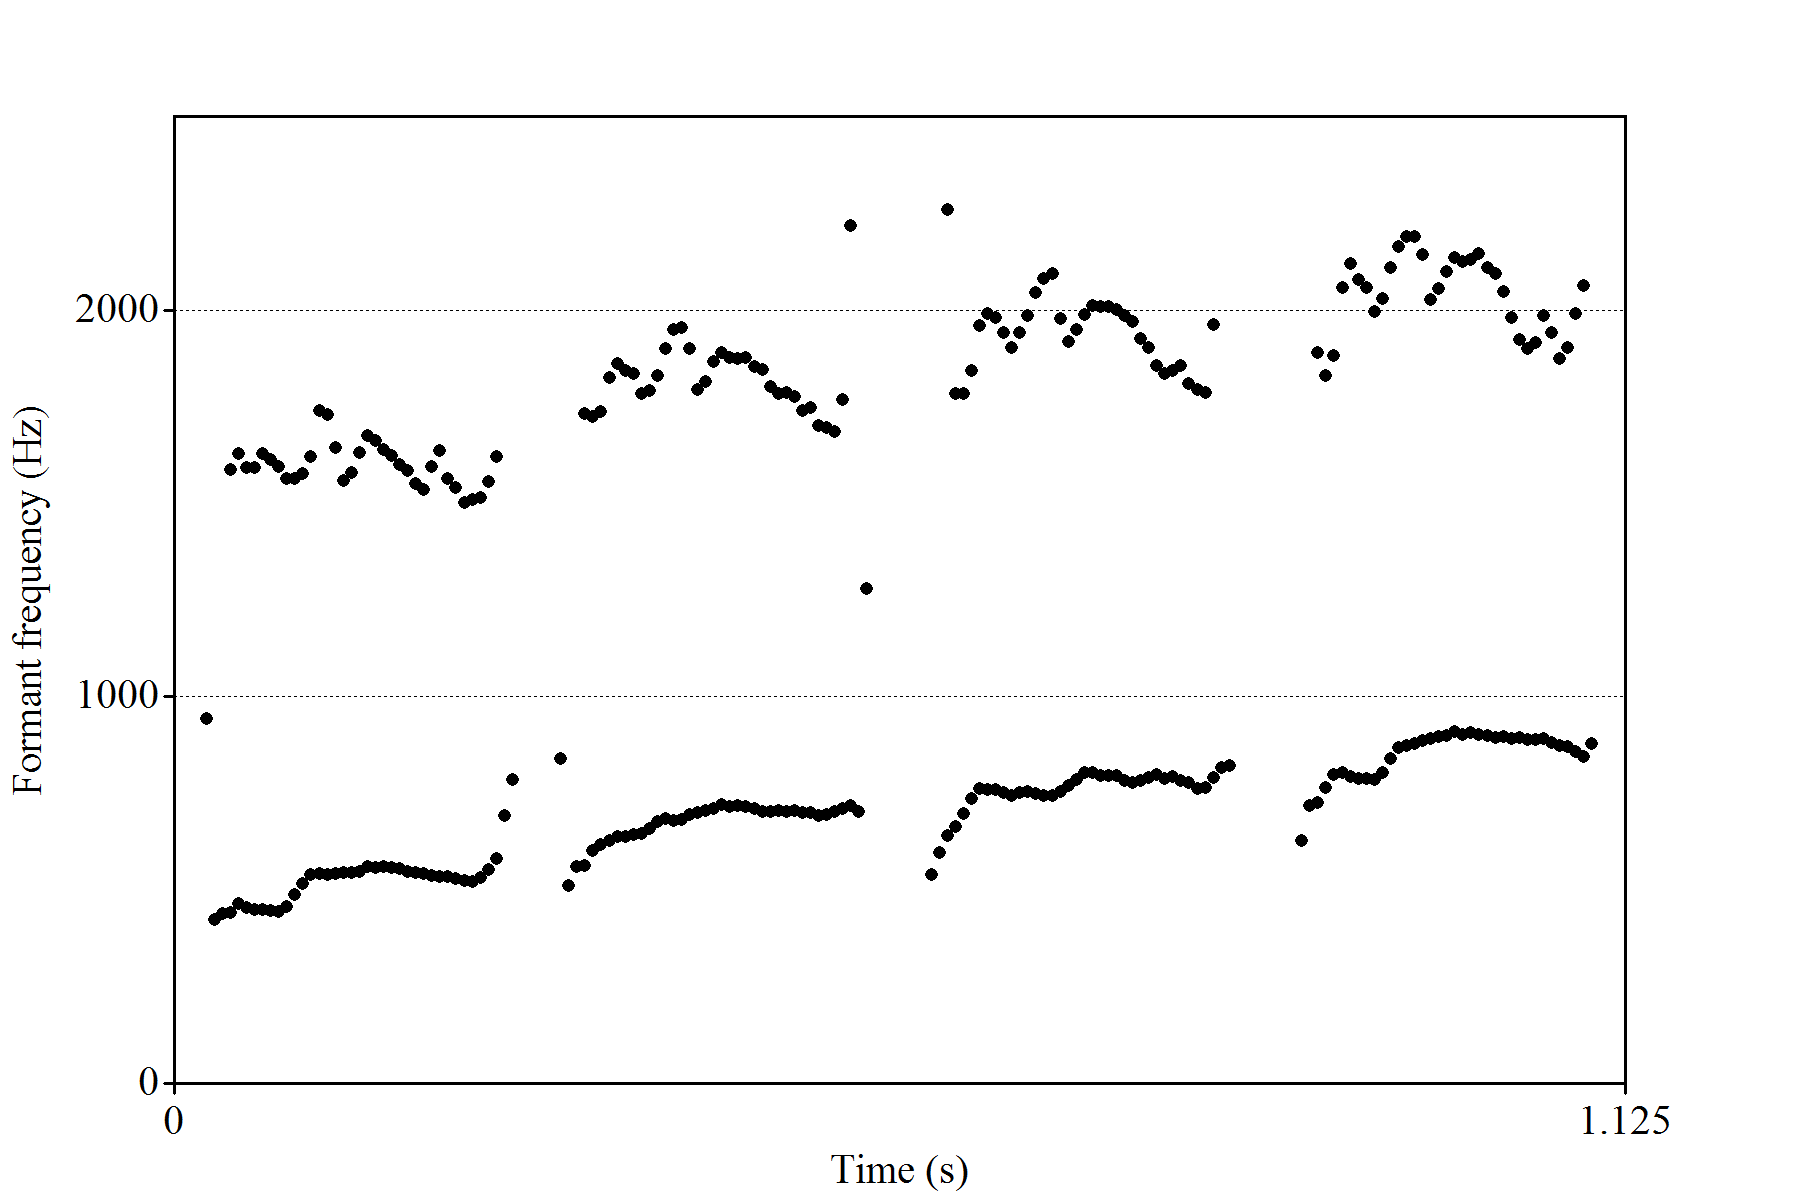
\includegraphics[width=0.75\textwidth]{./figures/fur_spectrogram.png}
	\caption{Formant tracks of \emph{fur} tokens}
	\label{fig.fur.spec}
\end{figure}

Table \ref{tab.vowel.stimuli} summarises the final parameters, and Figure \ref{fig.fur.spec} illustrates the result for one set of \textsc{nurse} tokens.
There was thus a continuum from stimulus 1 (hyper-Mancunian), to 2 (actual) and 3 (Scouse), to stimulus 4 (hyper-Scouse).
The formant structure of stimulus 2 was not modified, but still re-synthesis\is{resynthesis}ed so as not to stick out as the only completely natural recording.
For \textsc{nurse} stimulus 1 was thus higher and further back than the speaker's natural realisation, while stimuli 3 and 4 were both fronted and lowered to varying degrees.
With respect to happ\textsc{y}, stimulus 1 was lowered and centralised, while stimuli 3 and 4 were higher and fronter than the vowel that actually occurred in the recordings.
Participants always heard the re-synthesis\is{resynthesis}ed words in the same order (1 to 4).
Unfortunately, it was not possible to synthesis\is{resynthesis}e stimuli of satisfactory quality from the sentences that had happ\textsc{y} in phrase-final position (where it was typically realised as [ə], and often articulated with breathy voice).
For this reason, answer tokens for these sentences were taken from the equivalent recordings where happ\textsc{y} occurred in the middle of the sentence (and in the same carrier word).
Crucially, however, the realisation of happ\textsc{y} in the stimulus sentence itself was not altered.
With hindsight, this should have been avoided as this procedure created a confound with the independent variable `position of keyword in sentence' (cf. Section \ref{sec.perc_res.happy}).

\subsection{Consonant stimuli}\label{sec.perc_method.con}

An equivalent procedure was developed for the consonants /ŋ(g)/ and /k/.
The link between those two in the context of this study is that the proportion of friction/aspiration is higher in the Scouse than in the standard British English variants, and this criterion was used to build a continuum similar to the one created for the two vowels.
Once more, the goal was to create roughly equal \isi{perceptual distance} (again checked auditorily by the author) between any two tokens, just as for the re-synthesis\is{resynthesis}ed vowels.
For every keyword a TextGrid was prepared which marked phases of aspiration, burst, and silence (for /k/) or nasality (for /ŋ(g)/) respectively (cf. Figure \ref{fig.chicken.spec}).
For /ŋ(g)/, a script written by the author of this study then

\begin{enumerate}
	\item cut away the aspiration for stimulus 3,
	\item additionally cut away the burst for stimulus 2 (leaving only the nasal),
	\item and shortened the (often rather long) nasal by 25\% to arrive at a more standard-like length for stimulus 1.
\end{enumerate}

\begin{figure}[h]
	\centering
	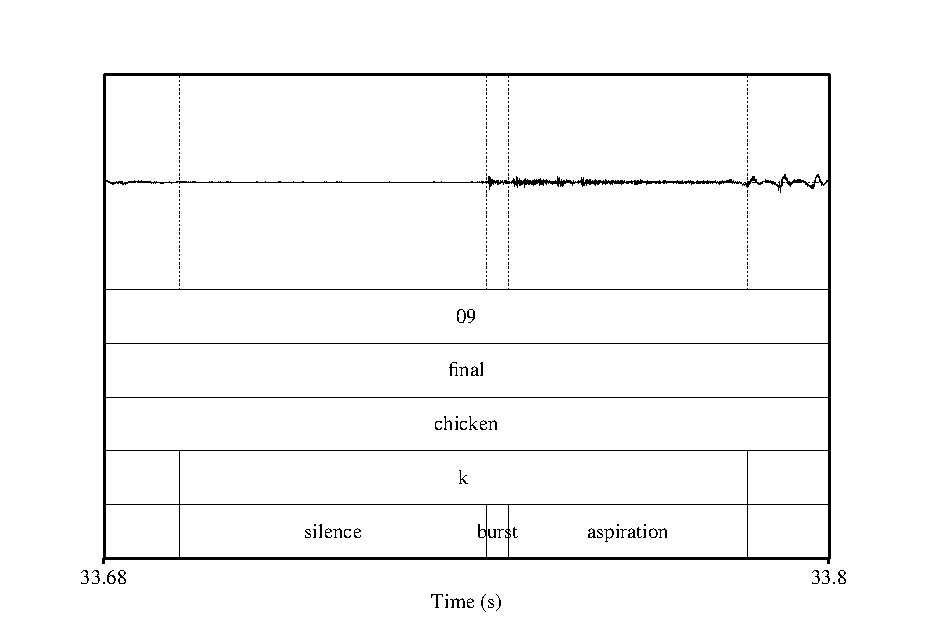
\includegraphics[width=0.75\textwidth]{./figures/chicken_spectrogram}
	\caption{Waveform and TextGrid for \emph{chicken} stimuli}
	\label{fig.chicken.spec}
\end{figure}

Stimulus 4 was the full, unaltered velar nasal plus realisation [ŋg].
To make the velar nasal plus sentences comparable to those of the other variables, stimulus 2 was afterwards copied back into the sentence to replace the natural [ŋg] realisation.
There was thus no voiced velar plosive present in the sentences subjects heard, and the continuum of stimuli was structured in the same way as those for the vowels and for /k/ in the sense that stimulus number 2 was the objectively most accurate choice that corresponded best to the sound actually used in the sentence.

Stimulus 2 for /k/ was the actual released plosive [k] as it occurred in the sentence recordings.
The hyper-Mancunian stimulus was created from this by cutting the aspiration, but leaving in the burst.
The speaker had also recorded all the /k/ sentences using the Scouse fricative variants.
The frication from these variants was pasted into the place of the original aspiration to form an affricate stimulus 3 (to make the result more natural sounding half of the closure phase was also deleted).
Stimulus 4, finally, had the whole plosive (silence, burst, and aspiration) replaced by the fricative by way of removing remaining silence and burst from stimulus 3.

For both /ŋ(g)/ and /k/, asymmetrical cross-fading and intensity adaptation was applied in intervocalic\is{phonological context} environments to create a smoother and less artificial transition from the nasal or the aspiration-less plosive to the following vowel in the hyper-Mancunian tokens (using a 25 milliseconds fade-in interval for the vowel and 50 milliseconds of overlap between phonemes when concatenating).
Table \ref{tab.consonant.stimuli} provides an overview of the consonantal stimuli.

\begin{table}
	\caption{Structure of consonant stimuli}
	\label{tab.consonant.stimuli}
	\centering
	\begin{tabular}{lll}
		\hline
		& /ŋg/ & /k/\\
		\hline
		stimulus 1 & nasal only (shortened) & plosive with burst\\
		stimulus 2 & nasal only & plosive plus burst \& aspiration\\
		stimulus 3 & nasal plus burst & plosive plus burst \& frication\\
		stimulus 4 & nasal plus burst \& aspiration & fricative\\
		\hline
	\end{tabular}
\end{table}

A small pilot study was run among linguists of the English Seminar at the University of Freiburg to make sure the stimuli (both the vocalic and the consonantal ones) were
\begin{inparaenum}[(a)]
	\item sufficiently natural-sounding, and
	\item equally distant from one another in perceptual terms.
\end{inparaenum}
This pilot study did not reveal any problems, so the investigation proper was carried out using these stimuli.

\section{Presentation}
\label{sec.perc_method.pres}

\subsection{Online platform}
\label{sec.perc_method.pres.platform}

The actual test was administered online using SoSciSurvey.de \parencite{sosci}, a professional tool for academic online surveys and questionnaires.
The platform uses flash to play audio and video files.
Although declining in importance, flash is still installed on most desktop and laptop computers (though not on tablets and smartphones) so the vast majority of potential subjects should have had no technical problems related to the website.
Nevertheless, participants first of all had to answer a filter question to make sure they had flash installed and activate\is{activation}d and could actually play the sound recordings.
Subjects were given the hint that they were going to hear the name of a type of bird and the questionnaire then used the flash plug-in to play a short sound file of the speaker saying \emph{raven}.
Participants then typed in the word they had heard.
Wrong answers to this test question prevented the user from progressing in the questionnaire.
Participants were randomly assigned to one of two groups.
The control group was (correctly) told that the speaker they were going to listen to was from Manchester.
The other group was led to believe that the speaker was from Liverpool (about 1 in 3 of the participants who lived outside of Liverpool actually believed this).
Depending on which group subjects had been assigned to, `Manchester' or `Liverpool' was displayed at the top of every page as a reminder (cf. Figure \ref{fig.online.screenshot}).

\begin{figure}[h]
	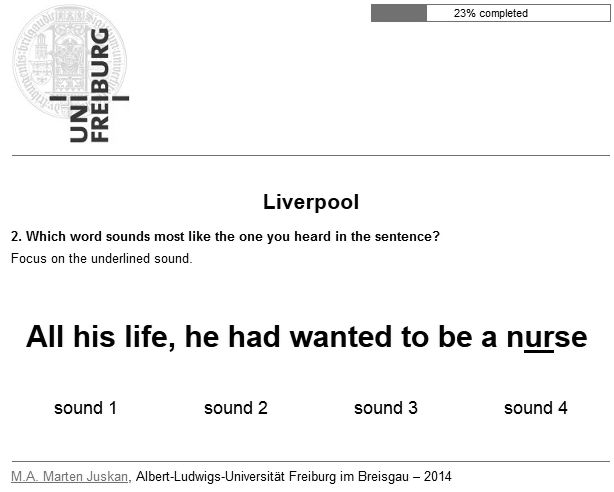
\includegraphics[width=\textwidth]{./figures/questionnaire_screenshot}
	\caption{Online questionnaire - training item}
	\label{fig.online.screenshot}
\end{figure}

After a couple of practice items (the results of which did not enter the analysis) participants were presented with 6 groups of 8 test tokens each.
Both the order of the groups and the order of the items within each group was randomised.
For every sentence, subjects were asked to pay special \isi{attention} to the (part of the) word that was underlined.
The sound files that were played had been created using another Praat script written by the author which pasted the stimulus sentence together with the resynthesis\is{resynthesis}ed keywords and added bits of silence in between (Figure \ref{fig.per.sentence} visualises the structure).

\begin{figure}[h]
	\centering
	
	\begin{tikzpicture}[->,>=latex,shorten >= 5pt,shorten <= 5pt, ultra thick, align=center, node distance = 2cm, on grid, main node/.style={rectangle,draw}]
	\small
	
	\node (A) {silence\\1.5s};
	\node[right = of A] (B) {carrier\\ sentence};
	\node[right = of B] (C) {silence\\1.5s};
	\node[right = of C] (D) {`one'};
	\node[right = of D] (E) {silence\\0.5s};
	\node[right = of E] (F) {token\\1};
	\node[below = of F] (G) {silence\\1.5s};
	\node[left = of G] (H) {`two'};
	\node[left = of H] (I) {silence\\0.5s};
	\node[left = of I] (J) {token\\2};
	\node[left = of J] (K) {silence\\1.5s};															
	\node[left = of K] (L) {`three'};
	\node[below = of L] (M) {silence\\0.5s};
	\node[right = of M] (N) {token\\3};
	\node[right = of N] (O) {silence\\1.5s};
	\node[right = of O] (P) {`four'};
	\node[right = of P] (Q) {silence\\0.5s};
	\node[right = of Q] (R) {token\\4};
	
	\draw (A) -- (B);
	\draw (B) -- (C);
	\draw (C) -- (D);
	\draw (D) -- (E);								
	\draw (E) -- (F);
	\draw (F) -- (G);
	\draw (G) -- (H);
	\draw (H) -- (I);
	\draw (I) -- (J);
	\draw (J) -- (K);
	\draw (K) -- (L);
	\draw (L) -- (M);
	\draw (M) -- (N);
	\draw (N) -- (O);
	\draw (O) -- (P);
	\draw (P) -- (Q);
	\draw (Q) -- (R);
	
	\node[below = 1cm of {$(O)!0.5!(P)$}] (cutoff) {RT\\cut-off point};
	\node[above = 1cm of {$(O)!0.5!(P)$}] (help) {};
	
	\draw[-, dashed] (cutoff) edge (help);
	
	\end{tikzpicture}
	
	\caption{Timing of perception stimuli}
	\label{fig.per.sentence}
\end{figure}

Each sentence was presented on a separate page of the questionnaire.
Participants would see the sentence first for 1.5 seconds before the playback started automatically.
After the recording of the sentence had finished playing, participants heard the four resynthesis\is{resynthesis}ed words (introduced by ``one'', ``two'', ``three'', ```four'' to avoid confusion\footnote{The token numbers were recorded by a different female speaker (aged 26). This was not ideal as it is possible that the accent of the other speaker might have influenced participants. Incidentally, however, \citeauthor{haydrager2010} were faced with the same problem and correctly point out that any effect the second speaker \emph{might} have had would manifest itself in identical fashion in \emph{both} experimental conditions and should therefore not be able to confound the \isi{priming} effect \parencite[cf.][871 and 889]{haydrager2010}.}) with 1.5 seconds of silence in between words, and were asked to choose the one that they thought corresponded most closely to the sound in the test sentence.
Participants could either choose a sound by clicking on a button or by pressing ``1'', ``2'', ``3'', or ``4'' on their keyboard.
Both the sentence and the resynthesis\is{resynthesis}ed sounds were only played once.
As soon as the subject had clicked on the button of their choice (or pressed the relevant key) the next sentence was automatically presented.

\subsection{Reaction times}
\label{sec.perc_method.pres.rt}

Reaction times were also recorded.
These have to be taken with a grain of salt in the context of an online survey, as a number of external factors (skill in using a mouse etc.) add a lot of variance.
The potentially most important factor --- speed of internet connection --- can be ruled out as a confounding variable, however.
This is because the platform uses JavaScript to send each subset of stimuli to the computer of the subject.
Playback of the sound files does not start before all bits of the question have been downloaded.
RT measurements (with an accuracy of about 10 milliseconds) are then taken locally on the participant's computer before being bundled and sent back to the server.
No loading from the server takes place in between stimuli \parencite[cf.][]{sosci}.
While there is still some room for variation between different hardware configurations in terms of timing accuracy and the like, there is no reason to assume that one subgroup of participants in particular would be affected in a significantly different way, so overall such unwanted effects can be hoped to cancel out.
Furthermore, reaction times were not analysed as a dependent variable in its own right, but `merely' served to filter responses in the way described below.

The platform \citetitle{sosci} does come with some technical limitations, however, since it is not primarily designed for tests requiring RT measurements.
Unfortunately, it is neither possible to define a time window outside of which participants cannot enter a response nor to specify when the reaction time clock starts.
Technically speaking, RT measurements are really measurements of how long a subject spent on a particular page of the questionnaire.
Measuring thus starts automatically once the page is loaded and stops when the next page is accessed (which, in this study, happened automatically once an answer had been selected).
``Real'' reaction times are arrived at by substracting the total duration of each audio file from the time spent on the respective page.

As a consequence of these restrictions, it was possible for subjects to make their choice at any time, including \emph{before} the recording had actually finished even though the instructions spelled out that participants should listen to all answer options first.
It would have been quite easy to filter out all of these premature answers by simply eliminating all observations with negative RTs from the dataset.
This course of action was not taken for two reasons.
The first one is comparability with previous research.
Neither \textcite{niedzielski1999} nor \textcite{hayetal2006b,haydrager2010} even recorded reaction times and responses were given on a physical answer sheet so it is quite possible that these studies were, in part, based on answers that had been given before subjects had listened to all of their options.
The second, more important reason, is that it does not necessarily make sense to exclude an answer just because the subject did not listen to all resynthesis\is{resynthesis}ed sounds first.
After all, this study is interested in finding out how (stereotypical\is{stereotype}) expectations influence people's perception.
The claim that at least some expectations and \isi{attitude}s will prime\is{priming} people to perceive particular sounds \emph{implies} that at least to a certain extent the choice is already made before subjects can really process the physical signal and this might well show in negative RTs.
Many people might simply be reluctant to wait for the end of the recording if they already `know' the answer or if they have already heard the option that they think is the best match.
Ignoring negative RTs might then result in involuntarily eliminating (parts of) the \isi{priming} effect one is interested in from the dataset --- which might be a reason why previous studies have not even bothered with reaction times in the first place.

On the other hand, it is fortunate if one is able to cleanse the dataset of nonsense answers which are particularly likely to occur in an online test where the physical presence of the researcher cannot act as an incentive to take the task at hand seriously.
Responses with RTs that indicate the subject did not even listen to the carrier sentence, let alone the answer options, are clearly nothing but noise and should be eliminated from the sample.
As a sort of compromise it was decided to keep all responses that were not given more than 2000 milliseconds before the end of the stimulus.
This threshold ensures that the participant has listened to at least three of the four answer options (cf. Figure \ref{fig.per.sentence}).
Responses that were given more than 4000 milliseconds after the end of the recording were likewise eliminated.

\section{Participants}\label{sec.perc_method.subjects}

Finding participants for the online test proved rather difficult.
Subjects were recruited through a number of channels.
A call for participants was distributed through Hope, Liverpool, and Manchester University.
Announcements posted in Liverpool and Manchester related groups on Facebook resulted in some (but very few) responses.
Some exchange students were recruited with the help of public notice boards on the campus of Freiburg University.
Several friends and colleagues were kind enough to spread the word via e-mail and social media, and this friend-of-a-friend approach proved to be comparatively fruitful.
Finally, personal contacts in Liverpool and Manchester and some of the people who had been interviewed about a year earlier were contacted and asked if they would like to participate.
All participants were required to
\begin{enumerate}
	\item be British
	\item be native speakers of English
	\item have normal hearing
\end{enumerate}
The necessity of the last requirement should be obvious, as subjects were supposed to choose between audio stimuli that differed in rather subtle ways.
Requirements 1 and 2 were set to make sure participants were at least likely to have some degree of experience with or knowledge of the accents of Liverpool and Manchester.
After all, \isi{exemplar} \isi{priming} can only work if there are \isi{exemplar}s that can be activate\is{activation}d by the prime\is{priming}.
Given what \textcite{montgomery2007} found with respect to the status of Scouse in particular it seems not too far fetched to assume that people with British nationality (and native competence of English) have at least some \isi{exemplar}s indexed for `Liverpool', even if these are only derived from (stereotypical\is{stereotype}) media perform\is{accent performance}ances.
People from, say, the U.S. or Australia, on the other hand, will probably be a lot less familiar with the British accent landscape and might not have the slightest idea of what a Scouse accent sounds like --- either because they have never listened to someone from Liverpool, or because they have not done so \emph{knowingly}, meaning that the relevant \isi{exemplar}s will be indexed for a more general category such as `British'.
In both cases, \isi{priming} subjects for `Liverpool' (or `Manchester', for that matter) would not be possible.

At the end of the questionnaire, participants had to indicate their age, gender, educational level, profession (profession of parents for students), geographical origin and current town/city of residence (both via the first half of UK postcodes), and whether they self-identified as working or middle class.
The occupation scale was the simplified version of the National Statistics Socio-economic Classification, which is used, for instance, by the \citeauthor{nomis} and classifies jobs into lower, intermediate, and higher, primarily based on how much routine (at the lower end) and responsibility over others (at the upper end) is involved.
Just as for the interview data, levels of occupation and education were then used to classify subjects as belonging to one of the two broad categories `working class' or `middle class'.
Since this classification correlated strongly with the social class participants had explicitly chosen anyway, self-reported social class membership was used as a predictor for statistical modelling (see below).

On the basis of the postcodes participants provided, geographic coordinates were obtained from \url{http://xposition.co.uk/geopostcode/}, and a euclidean distance value was calculated for every subject using the following formula:
\begin{equation}
d = \sqrt{(lon_L - lon_s)^2 + (lat_L - lat_s)^2}
\end{equation}
Where \(lon_L\) and \(lat_L\) are the longitude and latitude of central L1 (Liverpool city centre), \(lon_s\) and \(lat_s\) the (central) coordinates of the subject's postcode, and \(d\) is the resulting distance value (the higher, the further the subject lives from Liverpool).
These figures are not, strictly speaking, directly comparable.
This is because 1 degree of longitude translates to a different absolute distance in kilometres or miles depending on the latitude.
Since the north-south extent of the UK is comparatively small, however, the amount of distortion introduced was considered negligible.
Figure \ref{fig.per.subjects}\footnote{Map tiles by Stamen Design, under CC BY 3.0. Data by OpenStreetMap, under CC BY SA.} shows the geographical distribution of participants by representing every individual with a grey dot.
Two clusters are clearly visible, one in the north-west and one in the south-east of England.
The first is due to the fact that recruitment initially focussed on Liverpool and Manchester, while the London bias is to a degree even representative, given that between 15 and 20\% (depending on where one draws the boundaries) of the UK population live in the metropolitan area.
The remaining participants seem to come more or less from all over the country, although Wales and Northern Ireland are clearly under-represented.

\begin{figure}[h]
	\centering
	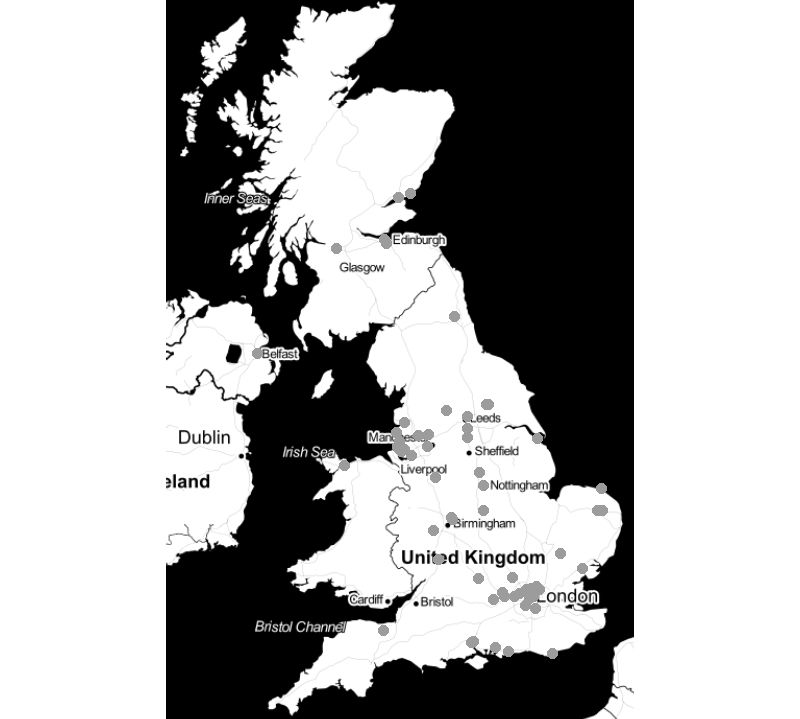
\includegraphics[width=0.49\textwidth]{./figures/participant_map}
	\caption{Geographical distribution of subjects (perception)}
	\label{fig.per.subjects}
\end{figure}

Subjects were given the opportunity to receive the results of the experiment after its completion and to participate in a lottery for a £100 gift card from a big online retailer.
E-mail-addresses were collected for these purposes, but kept strictly separate from the questionnaire responses (using an in-built function of the online platform specifically designed for that purpose).

In total, 67 subjects participated in the experiment and provided 2508 data points.
In addition to the more detailed placement via the postcode, participants were also assigned to one of the broad geographical categories ``internal'' (Liverpool and \isi{Merseyside}, ``L'' postcode area; 9 subjects) and ``external'' (everything else, 58 subjects).
It is possible that some of subjects in the Liverpool sample had already participated in one of the sociolinguistic interviews conducted by the author, but since these interviews had taken place (at least) a year earlier it is highly unlikely that this could have a distorting effect on results in the perception test.
Table \ref{tab.participants.perception} provides a more detailed overview of the `external' sub-sample (3 subjects in this group declined to indicate their gender).
One thing that is immediately obvious is that the middle class is heavily over-represented, only 7 subjects were classified as belonging to the working class.
Among middle class subjects, female and male participants are not really evenly distributed across \isi{priming} conditions: women dominate in the group that was prime\is{priming}d for Liverpool, while men do in the other.
However, Prime and Gender are still not collinear in the dataset (κ= 1.54), and mixed-effects ordinal models regressing reported percept on Gender did not find a significant effect of the latter, neither in the `Liverpool' (p = 0.801) nor in the `Manchester' condition (p = 0.597).
In other words, women and men did not behave differently in this experiment so the fact that they are unevenly distributed across conditions is unproblematic.
Incidentally, \textcite[69 and 79--80]{niedzielski1999} also found that \enquote{there was essentially no difference between what male and female respondents selected}.

\begin{table}[h]
	\caption[Gender and {social class} of subjects (perception)]{Gender and {social class} distribution of subjects (perception, external)}
	\label{tab.participants.perception}
	\centering
	\begin{tabular}{lcccc}
		\hline
		prime\is{priming} & \multicolumn{2}{c}{`Liverpool'} & \multicolumn{2}{c}{`Manchester'}\\
		& F & M & F & M\\
		\hline
		working class & 2 & 3 & 1 & 1\\
		middle class & 17 & 6 & 9 & 16\\
		\hline
	\end{tabular}
\end{table}

\section{Statistical analysis}\label{sec.perc_method.stats}

Unlike in the case of the interview data where there were fewer participants and the role of the individual subject was different (cf. Section \ref{sec.prod_method.stats}), it actually does make sense to include random effects for the statistical analysis of the perception data.

However, the data collected by the experiment described above are not ratio or interval scaled.
While answers are expressed in numbers (token 1, 2, 3, or 4), these are really labels for 4 distinct\is{distinctness} categories rather than measurements on a continuous scale.
There is no guarantee, for instance, that the (perceptual) distance from token 1 to token 2 is identical to that between tokens 2 and 3 (although this \emph{was} the aim when creating the tokens; cf. Sections \ref{sec.perc_method.vow} and \ref{sec.perc_method.con}) --- which is what the values suggest when they are being treated as numerical measurements.
On the other hand, the data \emph{are} ordered in a way (from most standard/Mancunian to most Liverpool), so while choosing token 4 instead of token 3 might not be the same as choosing 3 instead of 2 in terms of \isi{perceptual distance}, higher values do in all cases represent a more Liverpool-like percept than lower values --- much in the same way that, say, a higher RT always mean that a subject took more time to respond than another one with a lower RT.
It was therefore decided not to follow \textcite{hayetal2006a,haydrager2010} in treating the answers as numerical data for the purposes of statistical modelling.
Instead, the R package `ordinal' \parencite{Rordinal} was used to calculate cumulative link mixed ordered regression models via the Laplace approximation.

Subject was entered as a random intercept (cf. Section \ref{sec.prod_method.stats}), and a random by-subject slope for stimulus order was also included to counter any individual training or fatigue effects.
Carrier word was not included as a random effect because \isi{frequency} and, for consonants, phonological environment\is{phonological context} were of interest as fixed effects.
Since there were only 6 keywords per variable filtering out any lexical effects would almost certainly also have eliminated effects of \isi{frequency} and/or phonological environment\is{phonological context}.
Prime was entered as a fixed factor, along with gender, social class (self-reported), age of the subject, and \isi{geographical distance} from Liverpool.
Furthermore, the Zipf\is{Zipf score} score of the carrier word was included, as was the position of the carrier word in the stimulus sentence (sentence-medially or -finally), the position of the stimulus sentence within the experiment (when was the sentence played to the subject), and, for consonants, the phonological environment\is{phonological context} (V\_V or \_\#).
All two-way interactions of the prime\is{priming} with these linguistic and extra-linguistic factors were also considered.
Sum coding was used for all models in order to be able to identify main effects and interactions.
Model selection was based on AIC scores and F-tests comparing nested models.
Collinearity\is{collinearity} was investigated applying the functions written by Austin Frank (cf. Section \ref{sec.prod_method.stats}) to corresponding mixed-effects logistic regression models.